%\mychapter{6}{Results}

\section{Results}
In this section, we report our results on both synthetic and real-world data
using diffusion maps. We compare our results with those obtained via PCA, a popular linear dimensionality technique.

\subsection{Simulation results on Firing Rate}
In following sections, we show our fake-brain results using 
diffusion maps (DM) with l1 distance on simulated firing rate (SimFRDML1), and PCA  on simulated firing rate (SimFRPCA).


\subsubsection{DM on simulated FR data using L1 distance}

\begin{figure}[H]
  \centering
   \makebox[\textwidth]{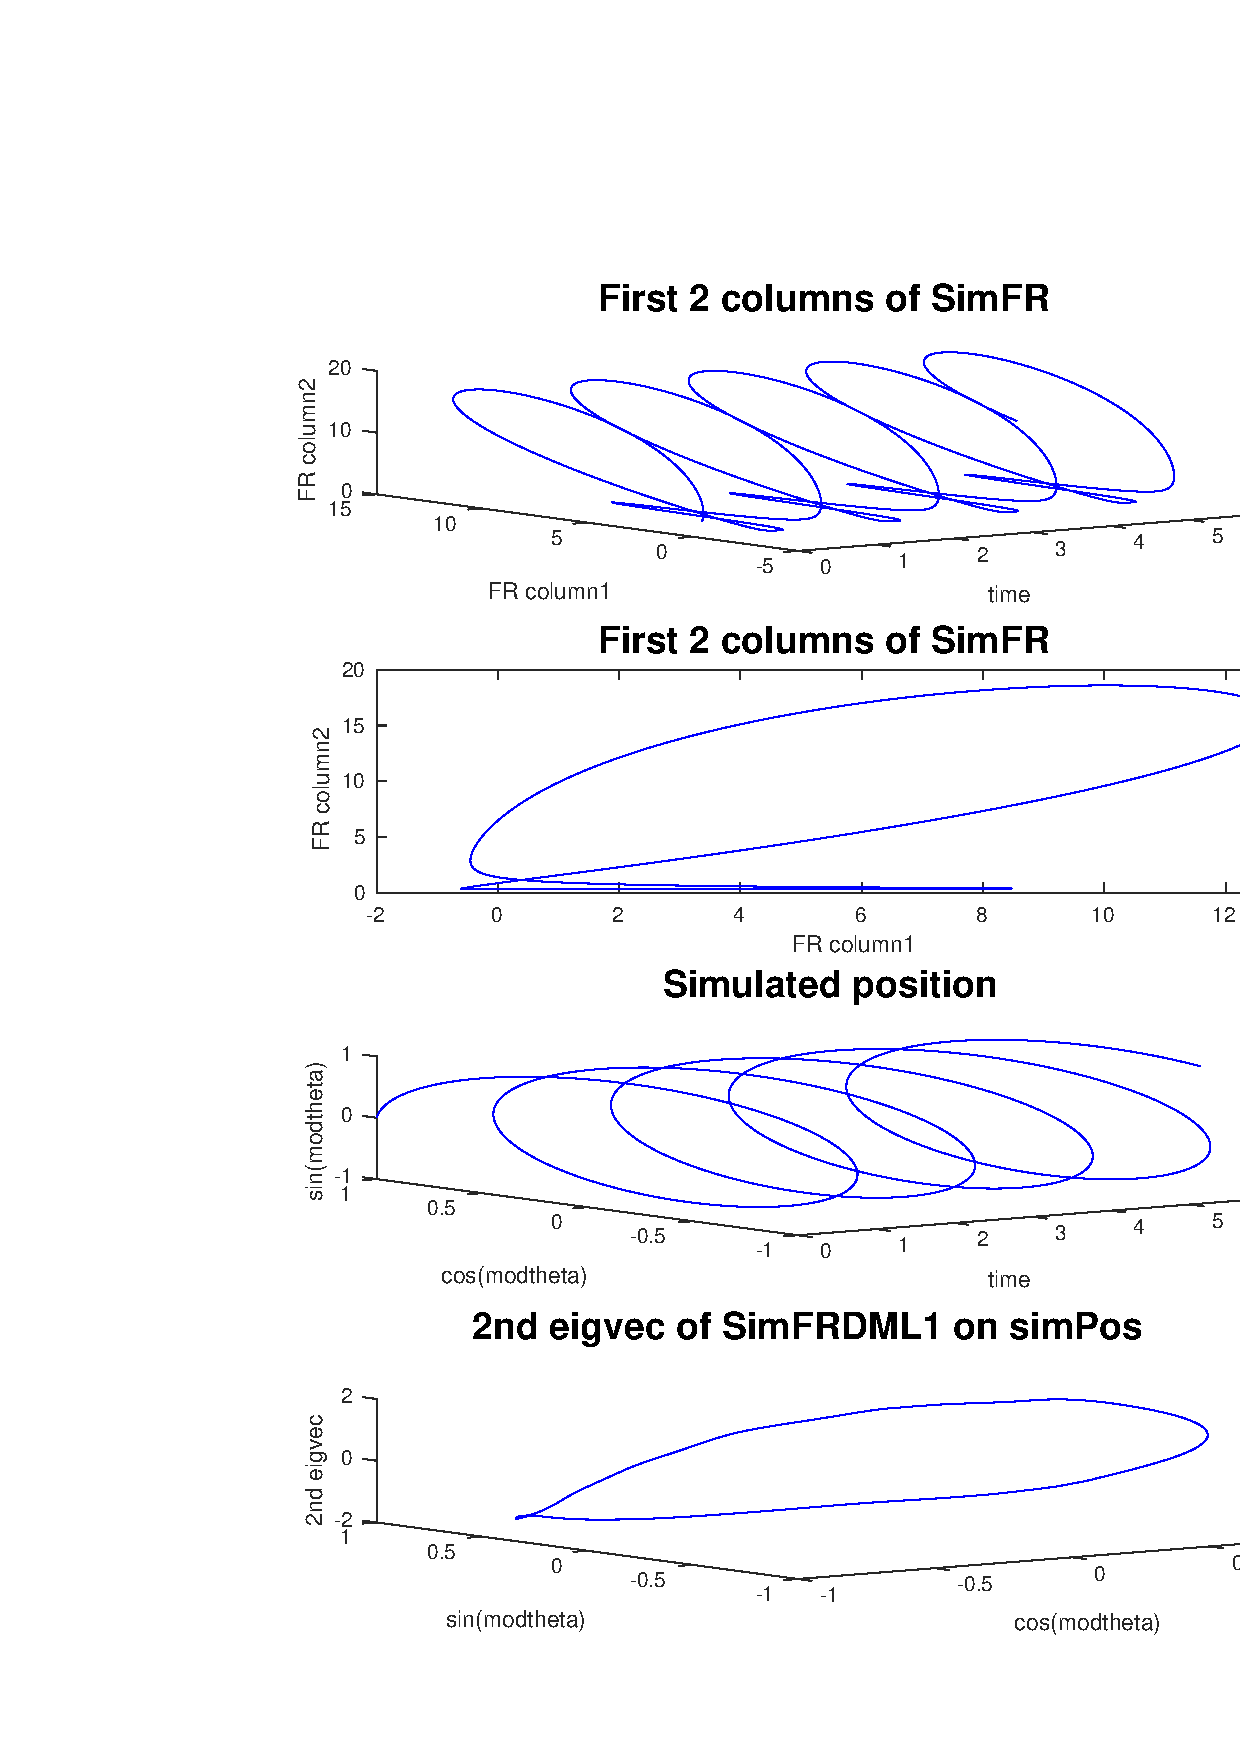
\includegraphics[width=\paperwidth]{/home/tesylvia/Oral_Sept_2017/images/FakeBrain-plots/DM-on-FR-L1.pdf}}
\end{figure}



\subsubsection{PCA on simulated FR  data}

\begin{figure}[H]
  \centering
   \makebox[\textwidth]{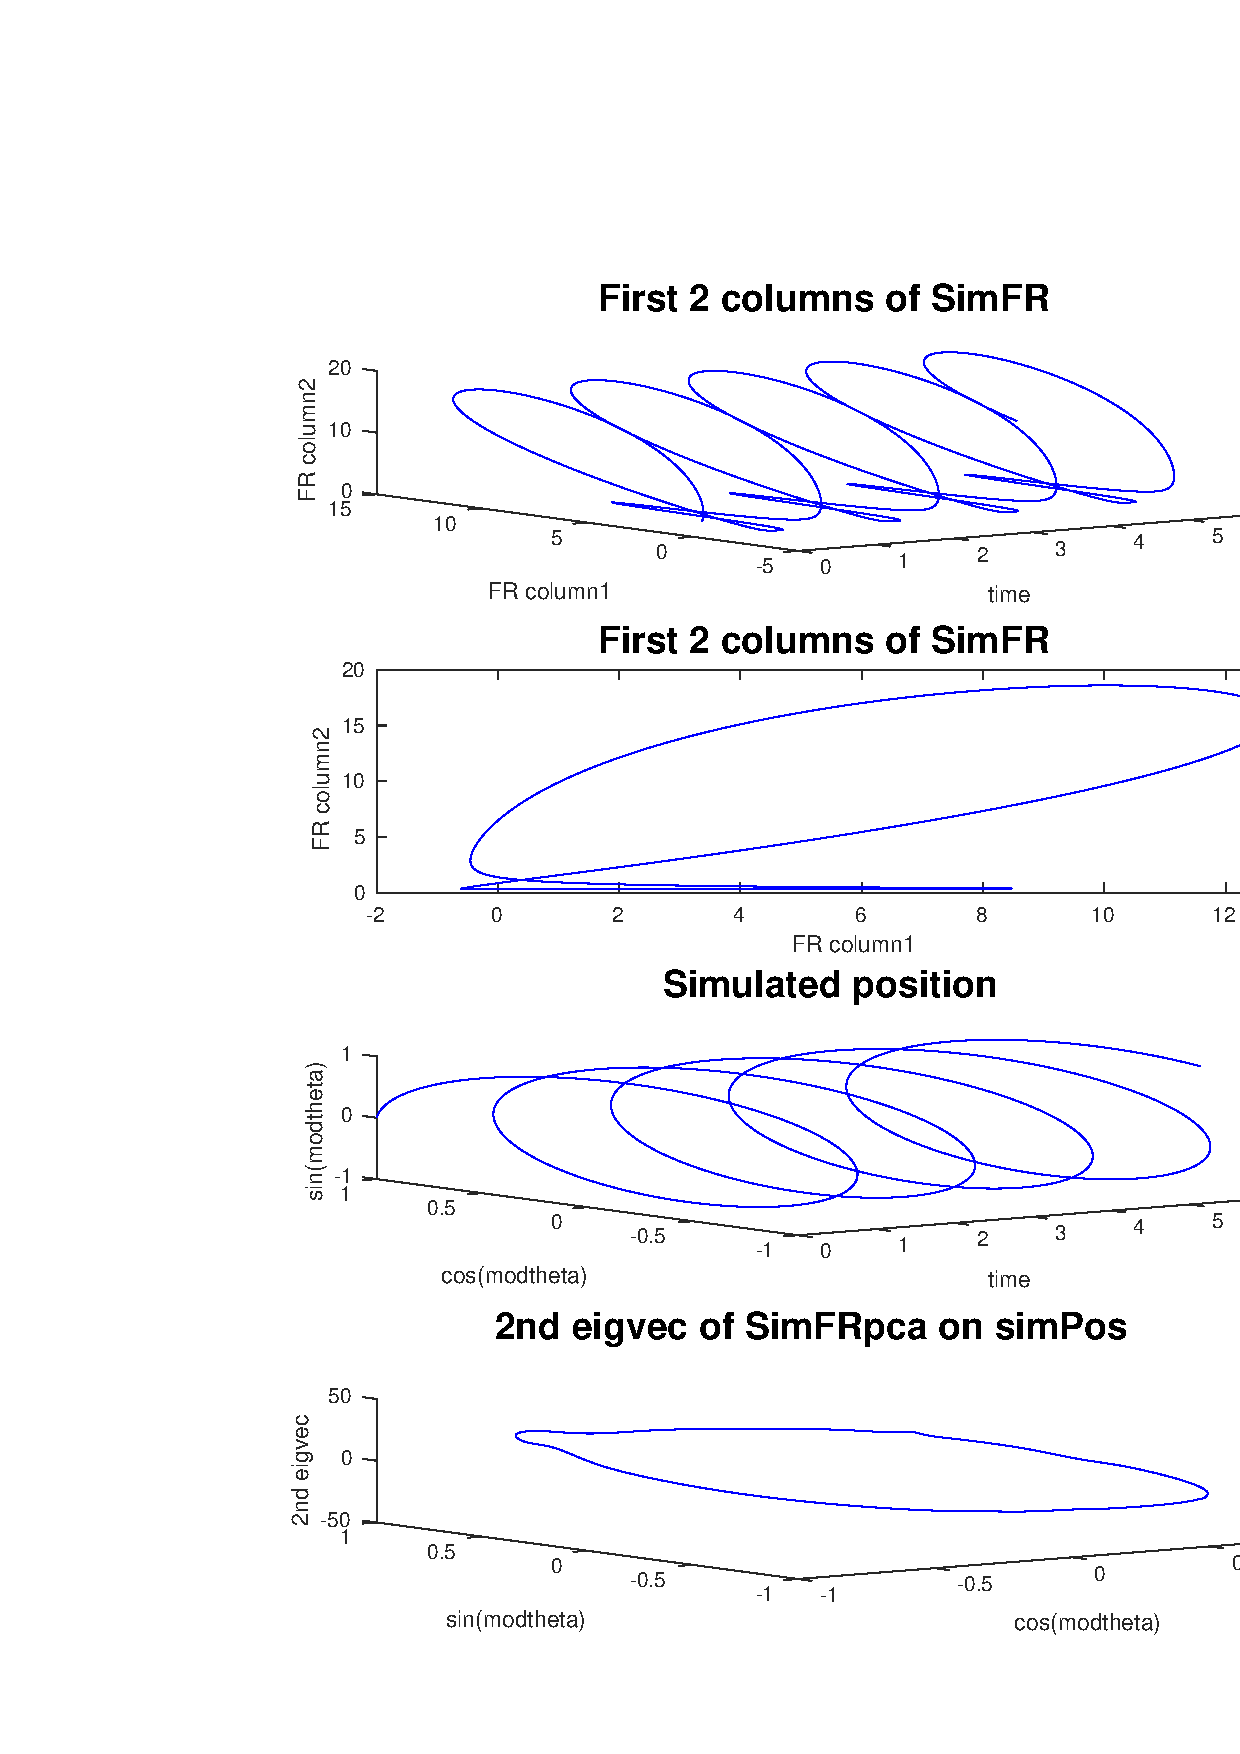
\includegraphics[width=\paperwidth]{/home/tesylvia/Oral_Sept_2017/images/FakeBrain-plots/PCA-on-FR.pdf}}
\end{figure}


\subsection{Simulation results on previous time data}
In these sections, we show our results of diffusion maps (DM),on simulated previous time (Simprevtime) using the l1 distance (SimprevtimeDML1)and  PCA on Simprevtime (SimprevtimePCA).



\subsubsection{DM on simulated prevtime data using L1 distance}

\begin{figure}[H]
  \centering
   \makebox[\textwidth]{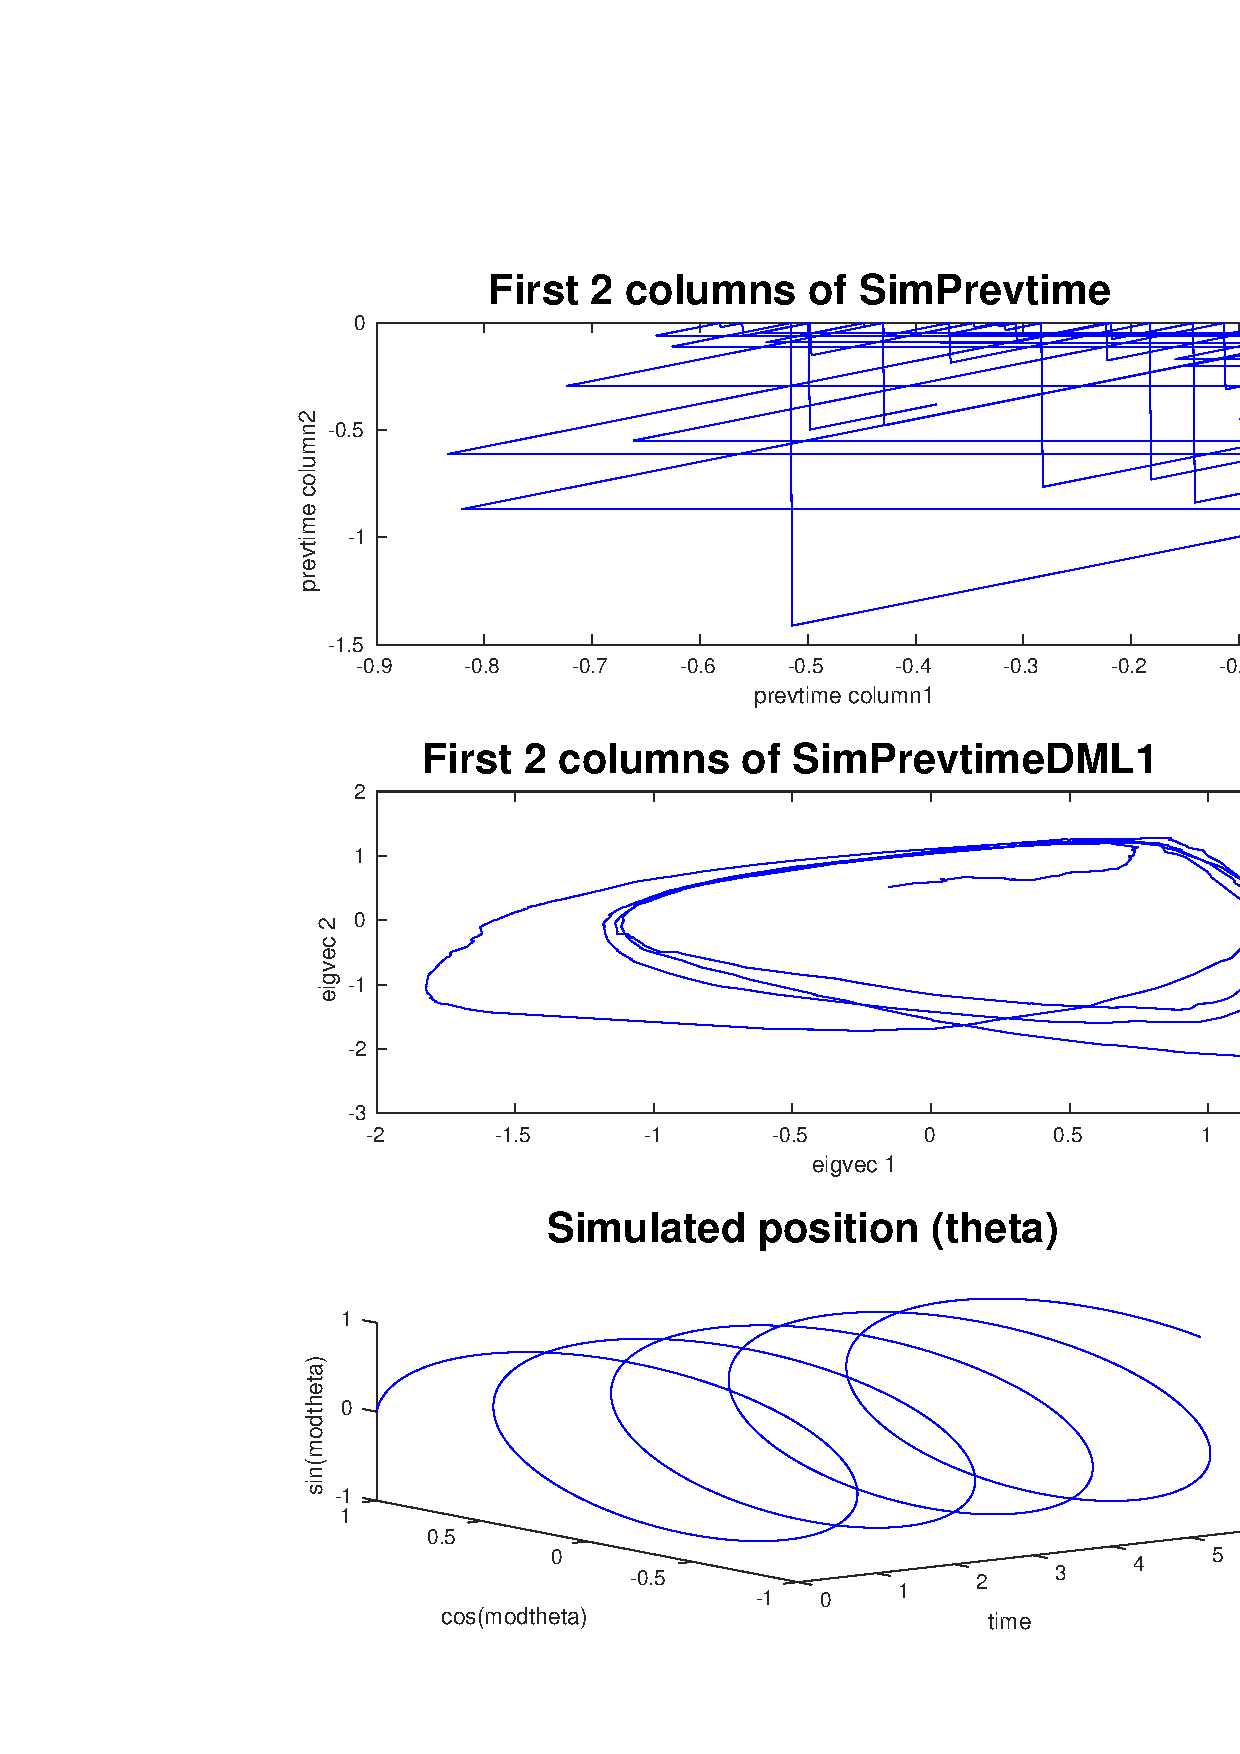
\includegraphics[width=\paperwidth]{/home/tesylvia/Oral_Sept_2017/images/FakeBrain-plots/FirstL1DM.pdf}}
\end{figure}



\begin{figure}[H]
  \centering
   \makebox[\textwidth]{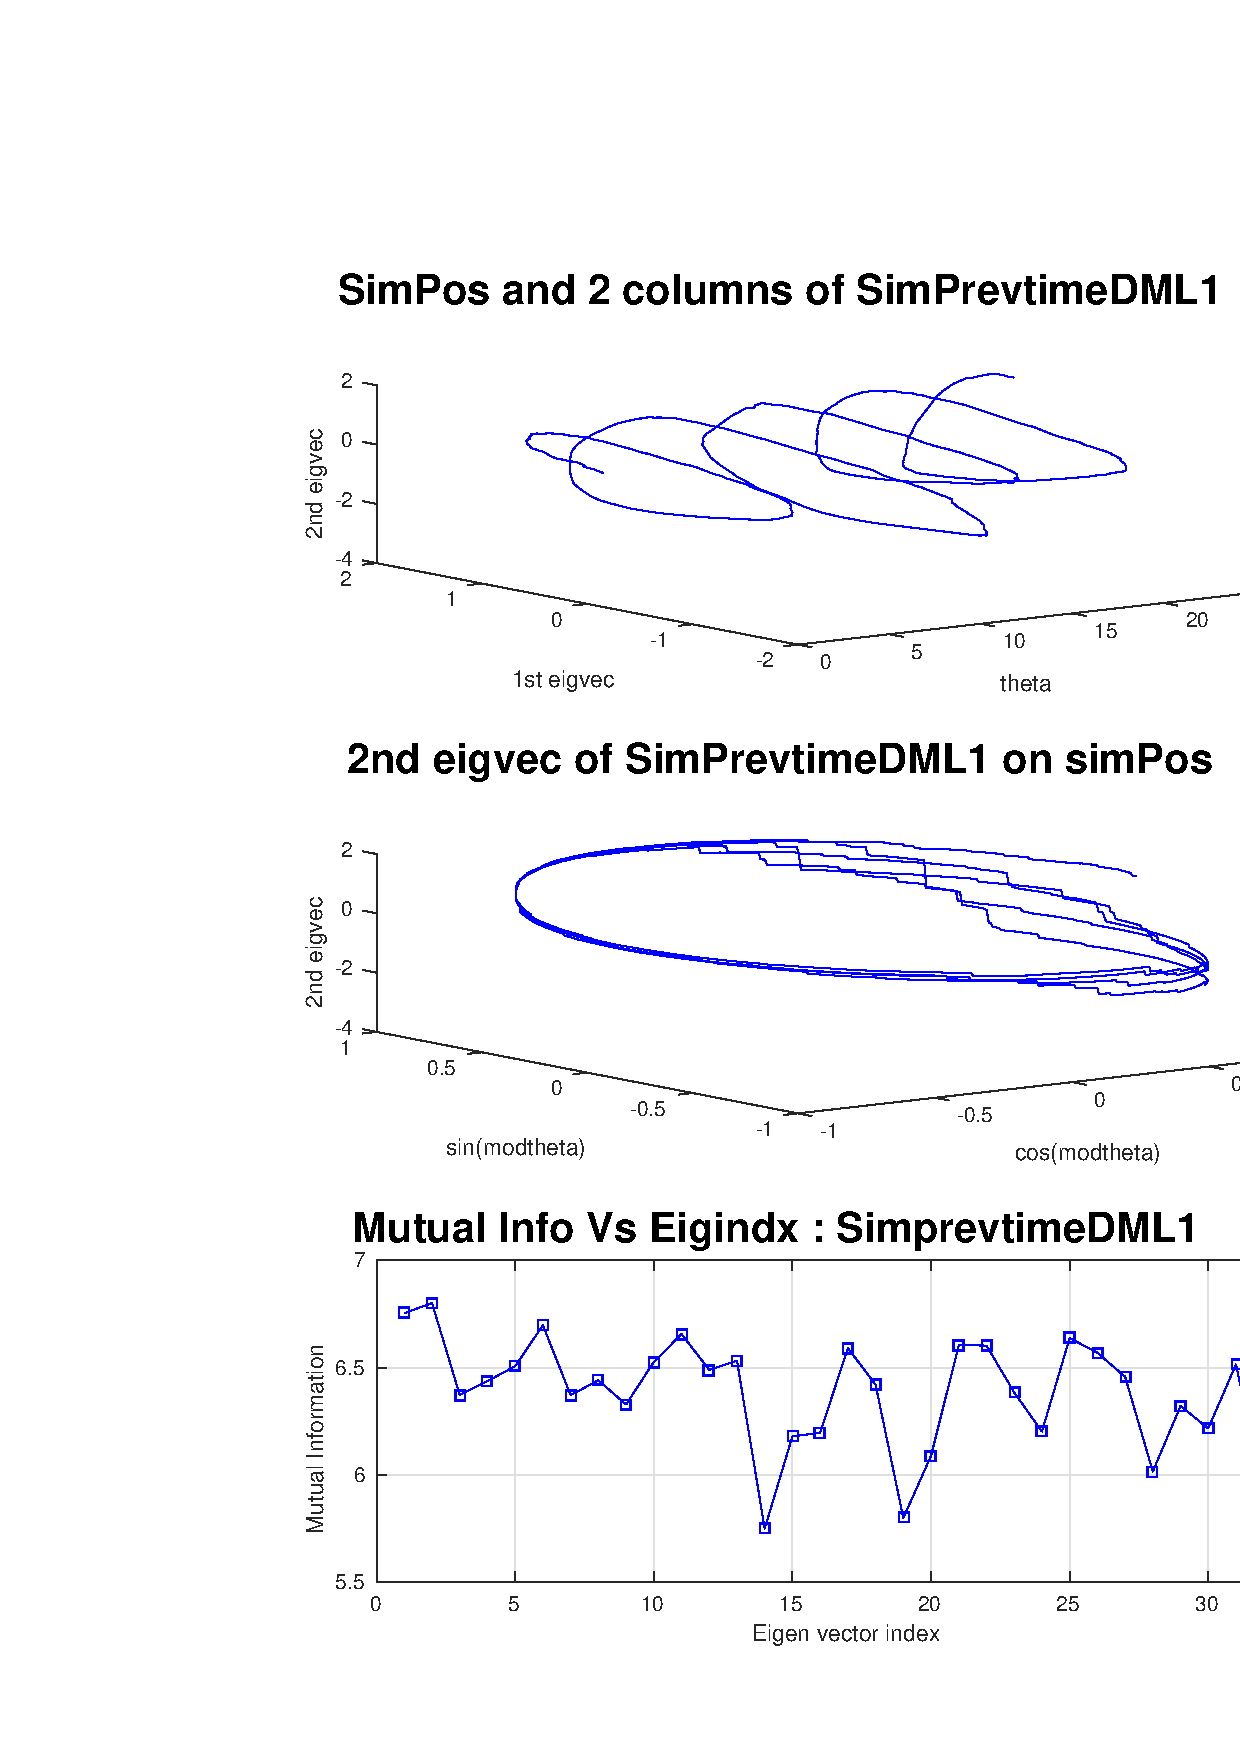
\includegraphics[width=\paperwidth]{/home/tesylvia/Oral_Sept_2017/images/FakeBrain-plots/SecondL1DM.pdf}}
\end{figure}




\subsubsection{PCA on simulated prevtime data}

\begin{figure}[H]
  \centering
   \makebox[\textwidth]{\includegraphics[width=\paperwidth]{/home/tesylvia/Oral_Sept_2017/images/FakeBrain-plots/FirstPCAMI.pdf}}
\end{figure}



\begin{figure}[H]
  \centering
   \makebox[\textwidth]{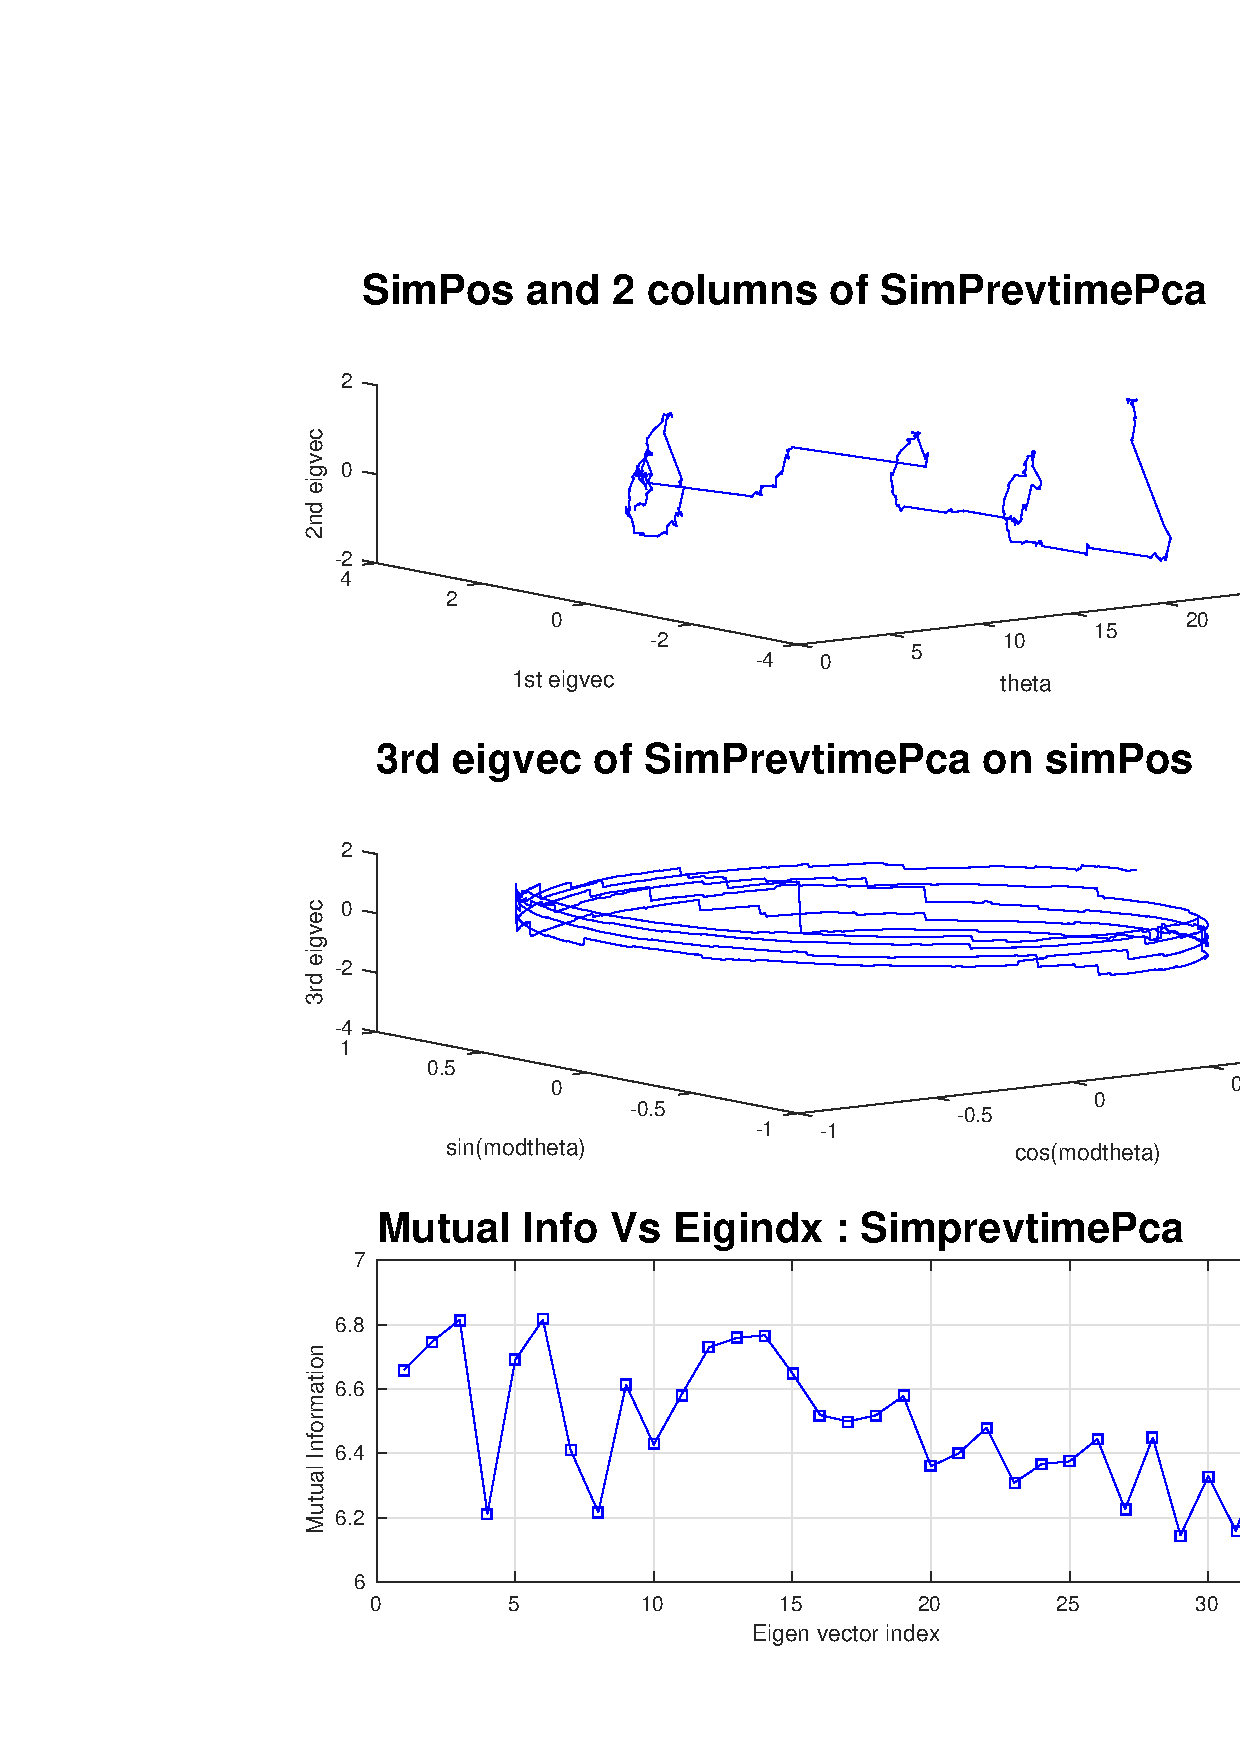
\includegraphics[width=\paperwidth]{/home/tesylvia/Oral_Sept_2017/images/FakeBrain-plots/MI-2PCA.pdf}}
\end{figure}




































































%\begin{itemize}
%\item show the graphs/results package
%\item this is how we're interpreting the results
%\item why does this matter?
%\item what measure of goodness did you use?
%(Fisher Vs Shannon information)

%%==========suggested by Duane============================================
%\item Mention that there are other ways of checking measures of goodness
% e.g the one provided by diffusion maps, Bayesian decoding refer to the nature
% and review artcicle.


%\end{itemize}







